\documentclass[compress,dvipsnames]{beamer}
\usepackage{amsmath}
%\usepackage[dvipsnames]{xcolor}
\usepackage{graphicx}
\usepackage{tikz}
%\usetikzlibrary{decorations.fractals}
\usepackage{caption}
\usepackage{adjustbox}
\usepackage{multirow}
\usepackage[utf8]{inputenc}
\usepackage{appendixnumberbeamer}
\usepackage{comment}
\usepackage{dsfont}
\usepackage{lipsum}
\let\olditem\item
\renewcommand\item{\olditem\justifying}
\usepackage{setspace}
\def\Put(#1,#2)#3{\leavevmode\makebox(0,0){\put(#1,#2){#3}}}

\definecolor{brightcerulean}{rgb}{0.11, 0.67, 0.84}

\hypersetup{urlcolor=links}


\usetheme[]{Boadilla}

\makeatother
\setbeamertemplate{footline}
{
  \leavevmode%
  \hbox{%
  \begin{beamercolorbox}[wd=.3\paperwidth,ht=2.25ex,dp=1ex,center]{author in head/foot}%
    \usebeamerfont{author in head/foot}\insertshortauthor
  \end{beamercolorbox}%
  \begin{beamercolorbox}[wd=.6\paperwidth,ht=2.25ex,dp=1ex,center]{title in head/foot}%
    \usebeamerfont{title in head/foot}\insertshorttitle
  \end{beamercolorbox}%
  \begin{beamercolorbox}[wd=.1\paperwidth,ht=2.25ex,dp=1ex,center]{date in head/foot}%
    \insertframenumber{} / \inserttotalframenumber\hspace*{1ex}
  \end{beamercolorbox}}%
  \vskip0pt%
}
%\setbeamertemplate{footline}[frame number]{}
%\setbeamertemplate{navigation symbols}{}
%\setbeamertemplate{footline}{}

\usepackage{bm}

\usepackage{ragged2e}
\usepackage{etoolbox}
\apptocmd{\frame}{}{\justifying}{}
\usepackage{ragged2e}
 
\newcommand{\onenormSize}[2]{#1\lVert#2#1\rVert_1}
\input macros.tex
\usepackage{mathtools}
\mathtoolsset{showonlyrefs}

\usepackage{amssymb}% http://ctan.org/pkg/amssymb
\usepackage{pifont}% http://ctan.org/pkg/pifont
\newcommand{\cmark}{\color{red}\text{\ding{51}}}%
\newcommand{\xmark}{\color{gray}\text{\ding{55}}}%
\newcommand{\ind}{\perp\!\!\!\!\perp}

\begin{document}


\begin{frame}[plain]

\title[Higher-order tensors]{\\
Nonparametric learning with matrix-valued \\
predictors in high dimensions}
\author{Chanwoo Lee, Miaoyan Wang\\
}
\date{}
\institute{
{
\vspace{.3cm}
\vspace{.2cm}
}
Summary of research work\\
 \vspace{.1cm}
{
\vspace{.1cm}
 June 1, 2020\\
\vspace{.1cm}
}

%\vspace{.1cm}
%\hspace{8cm}\includegraphics[width=2cm]{../figures/image.png}
%\\
}
\titlepage
\end{frame}




\begin{frame}{A successful story: Support vector machine (SVM)}

\centerline{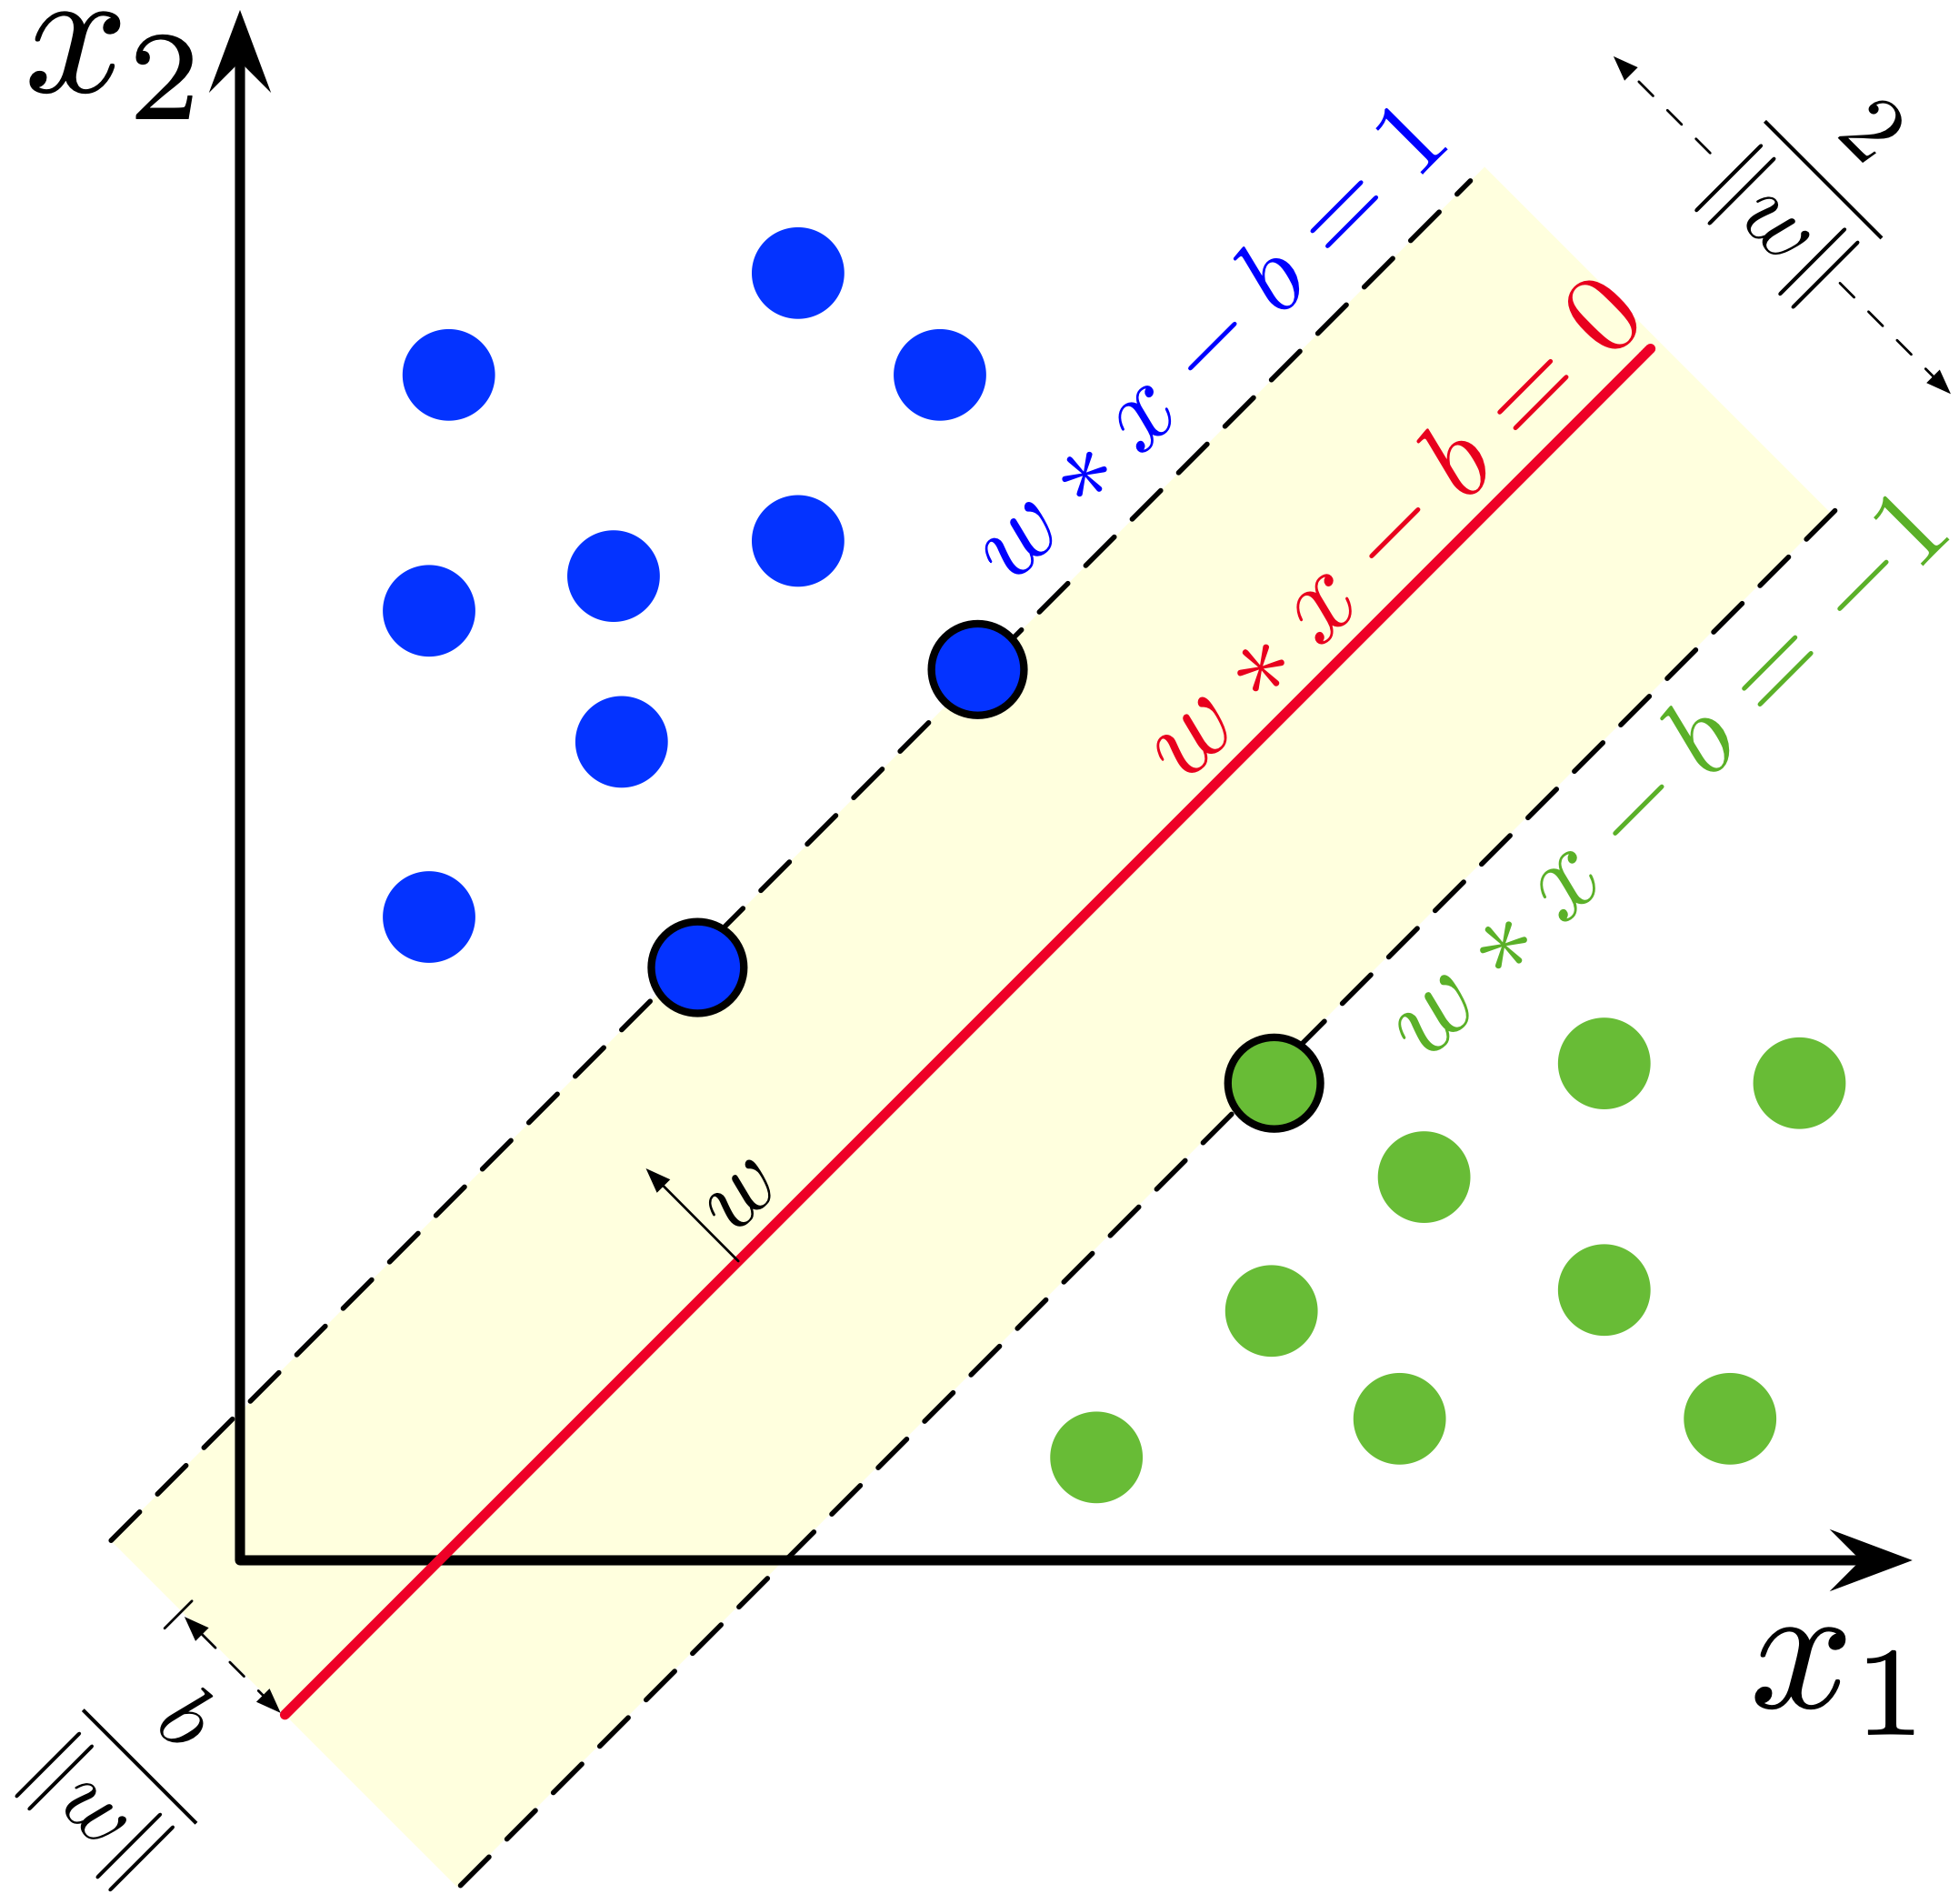
\includegraphics[width=.6\textwidth]{SVM_margin.png}}

Maximum-margin hyperplane for an SVM trained with {\color{red}2-d vector predictors} (Picture source: Wiki)
\end{frame}


\begin{frame}{SVM methods are powerful, however...}
\begin{itemize}
\item Input features are often expressed as {\color{red}matrices or tensor}  naturally rather than vectors
(ex. electroencephalogram (EEG), image classification).
\item How to {\color{red}efficiently classify high-dimensional matrices} with limited sample size: 
\[
n\ll d_1d_2 =  \text{dimension of feature space}\ ?
\]
\item How to {\color{red}robustly predict the label probability} when little is known about the function:
\[
\mathbb{P}(\text{Label $=1$} |\text{Matrix})\stackrel{\text{def}}{=}\mp(\text{Matrix}) \ ? 
\]
\item How to {\color{red}effectively reduce the sufficient dimensions} of the feature space without information lost:
\[
\text{Label} \ind \text{Matrix} | \phi(\text{Matrix}) \ ?
\]
\item For the purpose of presentation, we focus on {\color{red}matrix} predictors  and {\color{red}binary} outcomes.
\end{itemize}
\end{frame}


\begin{frame}{Previous methods for nonparametric multivariate learning}

\begin{table}
\resizebox{\columnwidth}{!}{
\begin{tabular}{c|c|c|c|c}
Method & SDR$^*$ & Robust prediction & Binary outcome & Tensor predictor\\
\hline
{\bf Weighted large-margin}&\xmark&\cmark&\cmark&\xmark\\
(Wang et al, JCGS'19)&&&&\\
(Zhang et al, JASA'10)&&&&\\
\hline
{\bf Deep Neural Network}&\xmark&\cmark&\cmark&\xmark\\
(...)&&&&\\
\hline
{\bf Principal SVM}&\cmark&\xmark&\xmark&\xmark\\
(Li et al, AOS'11)&&&&\\
(Shin et al, Biometrika'17)&&&&\\
\hline
{\bf Nonparametric regression}& \xmark&\cmark&\xmark&\cmark\\
(Imaizumi et al ICML'16)&&&&\\
\hline
\multirow{2}{*}{\bf Our method}&\multirow{2}{*}{\cmark}&\multirow{2}{*}{\cmark}&\multirow{2}{*}{\cmark}&\multirow{2}{*}{\cmark}
\end{tabular}
}
\end{table}
\vspace{1cm}
{\scriptsize $^*$SDR: sufficient dimension reduction. See later slides for definition.}
\end{frame}
%%%%%%%%%%%%%%%%%%%%%%%%%%%%%%%%%%%%%%%%%%%%%%%%%

\begin{frame}{Overview}
\tableofcontents
\end{frame}

\section{Motivation and Problem}
\begin{frame}{Motivational Problem}
Let $\{ (\mX_i, y_i) \in \mathbb{R}^{d_1\times d_2}\times \{-1,1\}\colon i=1,\ldots,n\}$ denote an i.i.d.\ sample from distribution $\tX\times \tY$. 
\begin{itemize}
\item (Probability estimation.) Estimate the conditional probability function
\[
\mathbb{P}(y^{\text{new}}=1|\mX^{\text{new}})={\color{red}p(\mX^{\text{new}})},
\]
where $p\colon \mathbb{R}^{d_1\times d_2}\mapsto [0,1]$ is the regression function of interest. 
\item (Sufficient dimension reduction, SDR.) Find a transformed predictor $\phi(\mX)$ such that
\[
y \ind \mX \large|{\color{red}\phi(\mX)},
\]
where $\phi\colon \mathbb{R}^{d_1\times d_2}\mapsto \mathbb{R}^{r_1\times r_2}$ is the dimension reduction of interest. 
\item Probability estimation concerns {\color{red}conditional mean}, whereas SDR concerns {\color{red}conditional independence} (stronger than mean). 
\end{itemize}
\end{frame}

\section{Linear Learning with low-rank kernels}
\subsection{Classification}
\begin{frame}{Key ingredient: low-rank support matrix machine (SMM)}
\begin{itemize}
\item Classification is an easier task than probability estimation. 
\item First, we develop a large-margin classifier for {\color{red} matrix predictors in high dimensions}.
\item Consider the classifier, $\hat g(\mX) = {\color{red}\text{sign}}\{\hat f(\mX)\}$, where $\hat f(\cdot)\colon \mathbb{R}^{d_1\times d_2}\mapsto \mathbb{R}$ is the solution to the following optimization over a function class $\tF$:
\begin{equation}\label{eq:SMM}
\hat f = \argmin_{f\in\tF}\left\{\sum_i \left[1-y_i f(\mX_i)\right]_{+}+\lambda\FnormSize{}{f}^2\right\}.
\end{equation}
Here$^{*}$ $\tF=\{f\colon f(\cdot)=\langle\cdot,\ \mB \rangle \text{ where $\text{rank}(\mB)\leq r$}\}$ and $\FnormSize{}{f}^2\stackrel{\text{def}}{=}\FnormSize{}{\mB}^2$.
\item Assume $r$ is fixed and known (for now). The classifier~\eqref{eq:SMM} is referred to as {\color{red}low-rank support matrix machine (SMM)}. 
\end{itemize}

{\scriptsize $^*$For presentation convenience, we omit the intercept $b$ in the representation of $f$.}
\end{frame}

\begin{frame}{Key ingredient: low-rank SMM}
\begin{itemize}
\item The proposed low-rank SMM finds the {\color{red}most separable hyperplane} among {\color{red}all possible $r$-dimensional representations}. 
\item Note that the low-rank SMM
\[
\min_{{\color{red}\text{rank}(\mB)\leq r}} \left\{\sum_i\left[ 1- y_i\left\langle \KeepStyleUnderBrace{\mX_i}_{\text{ambient dimension $d_1\times d_2$}}, \mB\right\rangle\right]_{+}+\lambda\FnormSize{}{\mB}^2\right\}.
\]
is equivalent to
\[
\min_{\substack{\mP_r\mP^T_r=\mP_c\mP^T_c=\mI_r \\ {\color{red}\mC\in\mathbb{R}^{r\times r}}}} \left\{\sum_i\left[ 1- y_i\left\langle \KeepStyleUnderBrace{{\color{red}\mP_r}\mX_i{\color{red}\mP^T_c}}_{\text{intrinsic dimension $r\times r$}}, {\color{red}\mC}\right\rangle\right]_{+}+\lambda\FnormSize{}{\mC}^2\right\},
\]
where $\mP_r\in\mathbb{R}^{r\times d_1}, \mP_c\in\mathbb{R}^{r\times d_2}$ are row- and column-wise projections, respectively. 
\end{itemize}
\end{frame}

\begin{frame}{Key ingredient: low-rank SMM}
\begin{itemize}
\item The solution to the low-rank SMM is represented as
%\[
%\hat \mB=\sum_{i=1}^n\hat \alpha_iy_i\KeepStyleUnderBrace{{\color{red}\hat \mP_c^T\hat \mP_c}\mX_i {\color{red}\hat \mP^T_r\hat \mP_r}}_{\text{rank $\leq r$}},\quad \text{and}\quad \hat f (\mX)\stackrel{\text{def}}{=}\langle \mX, \hat \mB \rangle,
%\] 
\begin{align}
\hat f(\mX)&=\sum_{i}\hat \alpha_i y_i\langle {\color{red}\hat \mP_r}\mX_i,\ {\color{red}\hat \mP_r }\mX \rangle,
%&=\sum_{i}\hat \beta_i y_i\langle \mX_i{\color{red}\mP_r},\ \mX{\color{red}\mP_r} \rangle
\end{align}
where $\{\hat \alpha_i\}$ are estimated (sparse) coefficients in the dual problem and $\hat \mP_r$ is the estimated projection matrix. 
\item We develop an alternating minimization algorithm to jointly estimate $\mP_r$ and $\{\alpha_i\}$. (The projection $\mP_c$ is absorbed into $\{\alpha_i\}$)
\item We are particularly interested in the high-dimensional regime when both $n$ and $\min\{d_1,d_2\}\to \infty$ while $r=\tO(1)$. {\it \scriptsize(An illustration of failures for classical SVMs in high dimensions; JMLR 18(45), 1-21, 2017).} 
\item The {\color{red}low-rankness} efficiently prevents overfitting in high dimensions.
 \end{itemize}
\end{frame}

\begin{frame}{Theory: Low-rank SMM in high dimensions}

\begin{itemize}
\item Let $\langle \cdot,\ \cdot \rangle_{\mP}$ denote the rank-$r$ projection kernel for a pair of matrices:
\[
\langle \mX, \mX' \rangle_{\mP}\stackrel{\text{def}}{=} \langle {\color{red}\mP} \mX,\ {\color{red}\mP} \mX'\rangle, \quad \text{for all }\mX, \mX'\in\mathbb{R}^{d_1\times d_2},
\]
where $\mP\in \mathbb{R}^{r\times d_1}$ is a (unknown) rank-$r$ projection matrix.
\item The low-rank SMM considers the decision function of the form:
\begin{align}\label{eq:f}
f(\cdot)=\sum_{i=1}^n \alpha_i y_i {\color{red}\langle \mX_i,\ \cdot \rangle_{\mP}}.
\end{align}
\item The function $f\in \tF_r$, where $\tF_r$ is the reproducing kernel Hilbert Space (RKHS) induced by rank-$r$ kernels $\{\langle \cdot,\ \cdot\rangle_{\mP}\colon {\text{projection }} \mP\in\mathbb{R}^{r\times d_1}\}$. 
\item Column-wise projection kernel can be similarly introduced $\Rightarrow$ same decision function. {\it A coincidence or something fundamental?} {\color{blue} May be because of rank theorem: r columns are enough to explain structure of  matrix X, by the same way r rows are enough for information of the matrix}
\end{itemize}
\end{frame}

\begin{frame}{Theory: Low-rank SMM in high dimensions}

\begin{block}{Generalization bound (Lee and Wang, 2020+)}
With probability at least $1-\delta$, the generalization error of low-rank SMM is
\[
\mathbb{P}\{Y^{\text{new}}\neq \text{sign}[\hat f(\mX^{\text{new}})]\} \leq \text{training error} +\mathbb{E}[\hat R_n(\tF_r)]+\sqrt{\ln({1\over \delta})\over 2n},
\]
where $\hat R_{n}(\tF_r)$ denotes the Rademacher complexity of rank-$r$ SMM classifiers. Roughly, in the case $d_1\asymp d_2=\tO(d)$, we have
\[
\mathbb{E}[\hat R_{n}(\tF_r)] \leq 4\varepsilon+{c_1{\color{red}r} \over \sqrt{n}} \int_{\varepsilon}^{\infty}\log^{1/2} \left({{\color{red} d/r}\over c_2\varepsilon'} \right)d\varepsilon',
\]
where the bound increases with {\color{red}$d$ and $r$}. Results highlight the role of $r$ in preventing overfitting. 
\end{block}



{\scriptsize \it 1. Check the proof more carefully; 2. consistency for relative risk. \\

See Varshney, K.R. and Willsky, A.S., IEEE Trans. Signal Process., 59(6), 2496-2512, 2011.}

\end{frame}


\begin{frame}{From classification to regression}
Back to the probability estimation problem. 
\begin{itemize}
\item Consider a piecewise-constant representation of the target probability function $p(\mX)\stackrel{\text{def}}{=}\mathbb{P}(Y=1|\mX)$:
\[
p(\mX) \approx {1\over H}\sum_{h\in[H]}{\color{red} \mathds{1}\left\{\mX\colon p(\mX)\leq {h\over H}\right\} },
\]
where $H\in\mathbb{N}_{+} \to \infty$ is the smoothing parameter. 
\item The classification problem has provided candidate decision regions:
\[
 \mathds{1}\left\{\mX\colon \KeepStyleUnderBrace{\text{sign}\left[\hat{f}_{h}(\mX)\right]=-1}_{\text{decision region from classification}}\right\} \stackrel{\text{in $p$}}{\longrightarrow} \mathds{1}\left\{ \mX\colon \KeepStyleUnderBrace{\mathbb{P}(Y=1|\mX)\leq {h\over H}}_{\text{target sublevel set}} \right\},
\]
for any $h=1,\ldots,H$.
\item This suggests a non-parametric approach to estimating $p(\mX)$.
\end{itemize}
\end{frame}


\subsection{Probability function estimation}
\begin{frame}{Algorithm}

We develop the following algorithm to solve for the target function: 
\begin{itemize}
\item Step 1. Choose a sequence of weights $\pi_h = {h\over M}, \text{for }h=1,\ldots,H$.
\item Step 2. For each weight $\pi_h\in[0,1]$, solve the following {\color{red}weighted low-rank support matrix machine (SMM)}:
\begin{align}\label{eq:sequence}
\hat \mB_h&=\argmin_{{\color{red}\text{rank}(\mB)\leq r}} \left\{\sum_{i}\omega_{\pi_h}(y_i)\left[1-y_i\langle \mX_i,\mB \rangle\right]_++\lambda\FnormSize{}{\mB}^2\right\},
\end{align}
\vspace{-2cm}
where $\omega_{\pi_h}(y) = 1-\pi_h$ if $y = 1$ and $\pi_h$ if $y =1$.
%Denote the optimal solution $\hat f_\pi (\mX)\stackrel{\text{def}}{=}\langle \mX, \hat \mB_\pi \rangle$.
\end{itemize}
\end{frame}

\begin{frame}{Algorithm (cont.)}
\begin{itemize}
\item Step 3. Denote the sequence of solutions and decision regions
\[
\hat f_h (\cdot)\stackrel{\text{def}}{=}\langle \cdot,\ \hat \mB_h \rangle \quad \text{and}\quad \hat \tD_h=\{\mX\colon\text{sign}[\hat f_h(\mX)] = -1 \},
\]
for all $h=1,\ldots,H$.
\item Step 4. Estimate the target probability function by
\begin{align}\label{eq:est}
\hat p(\mX)={1\over H} \sum_{h\in[H]} \mathds{1}\left\{\mX\in \hat \tD_h \right\}.
\end{align}

%\item 
%Step 4. Given a new feature $\mX^{\text{new}}$, predict the success probability by
%\begin{align}\label{eq:est}
%\hat f(\mX^{\text{new}})={1\over 2} (\pi^*+\pi_*),\quad 
%\end{align}
%where $\pi^*, \pi_*$ are the sign change points of the function $\hat f_h(\mX^{\text{new}})$ over the sequence of $\pi_1\leq \cdots \leq \pi_{M-1}$. That is,
%\begin{align}
%\pi^*&=\max\{\pi_h\colon \text{sign}(\hat f_h(\mX^{\text{new}}))=1,\ h\in[M-1]\},\\
%\pi_*&=\min\{\pi_h\colon \text{sign}(\hat f_h(\mX^{\text{new}}))=-1, h\in[M-1]\}.
%\end{align}
\end{itemize}
{\scriptsize \it The estimator~\eqref{eq:est} is asymptotically equivalent to the original estimator in Wang et al [Biometrika'08]. I choose this form because of its good analytic properties.}

\end{frame}



\begin{frame}{Theory: Probability prediction via low-rank kernels}
\begin{block}{High-dimensional consistency (Lee and Wang, 2020+)}
Assume the true $p\in \tF$, where $\tF$ is the RKHS induced by $\langle \cdot,\ \cdot\rangle_{\text{rank-r}}$. 
\begin{itemize}
\item Given any $\pi\in[0,1]$, the solution to~\eqref{eq:sequence} yields the Bayes rule:
\[
{\color{red}\text{sign}}[\hat f_\pi(\mX)] \stackrel{\text{in $p$}}{\longrightarrow} {\color{red}\text{sign}}[p(\mX)-\pi], \ \text{as }  n, d\to \infty \text{ while } {d/ n}\to 0.
\]
\item Our probability estimator~\eqref{eq:est} is consistent:
\[
\hat p(\mX) \stackrel{\text{in $p$}}{\longrightarrow} p(\mX), \quad \text{as}\ H, n,d \to \infty \text{ while } {d/n}\to 0.
\]
\end{itemize}
\end{block}

\begin{itemize}
\item To the best of our knowledge, this is the first result for SVM-based prob.\ estimation in large dimension ($d^2$), large sample size ($n$) regime. 
\item {\it \scriptsize Detailed proofs, assumptions? Convergence in terms of smoothness of $p$, $r$, $d$, $n$, and $H$? Do we really need the assumption, $p\in \tF$; i.e., $p(\cdot)$ linear in $\mX$? Perhaps not... composition of monotonic + linear functions is also fine.. indicator functions are dense in $L[0,1]^2$...}
\end{itemize}

\end{frame}

\subsection{Sufficient dimension reduction}
\begin{frame}{SDR via low-rank kernels}
\begin{itemize}
\item A challenging problem is to identify the {\color{red}sufficient features} with minimal modeling assumption in the prediction model. 
\item We develop a robust sufficient dimension reduction (SDR) method for matrix predictors in high dimensions. 
%\item The low-rank SMM algorithm lends itself well to the SDR problem. 
\end{itemize}

\vspace{.5cm}
We have SDR procedure based on  step 1 and 2 in Algorithm above.\\
Add two steps to Algorithm: 
\begin{enumerate}
\item Pre-step 2 (Whitening): $\mX_i \leftarrow \hat \Sigma^{-1/2}_{r}\left[\mX_i-\text{Mean}(\mX)\right]\hat \Sigma^{-1/2}_{c}$, where $\hat \Sigma_{r}, \hat \Sigma_{c}$ are empirical row- and column-wise covariance matrices.
\item Post-step 2(Assembling): Arrange outputs $\hat \mB_h$ into an order-3 tensor:
\[
\tB(\colon,\colon,h) \leftarrow \hat \Sigma^{1/2}_{r} \hat \mB_h \hat \Sigma^{1/2}_{c},\quad \text{for }h=1,\ldots,(H-1).
\]
Perform a rank-$(r_1,r_2,r_1r_2)$ Tucker decomposition on $\tB$. Let $\hat \mP_c, \hat \mP_r$ denote the estimated factor matrices at the first two modes. 
\end{enumerate}
\end{frame}



\begin{frame}{Theory: SDR via low-rank kernels}
\begin{block}{Bilinear sufficient dimension reduction (SDR)}
Let $(\mX,y)\in\mathbb{R}^{{\color{red}d_1\times d_2}}\times \{0,1\}$ be the pair of r.v.'s of interest.  Bilinear SDR seeks a pair of matrices $\mP_r\in\mathbb{R}^{r_1\times d_1}, \mP_c\in\mathbb{R}^{r_2\times d_2}$ such that
\[
y\ind \mX \big|\KeepStyleUnderBrace{\mX\times_1\mP_r\times_2\mP_c}_{\text{\color{red}$r_1$-by-$r_2$}}.
\]
The minimum dimension of $(r_1,r_2)$ is called the structure dimension. 
%We refer to the cartesian product of subspaces, $S_{Y|\mX}=\text{Span}(\mP_r)\times \text{Span}(\mP_c)$, as the bilinear central subspace. 
\end{block} 

\begin{block}{Unbiasedness (Lee and Wang, 2020+)}
Under suitable assumptions$^*$, our proposed $\hat \mP_r$ and $\hat \mP_c$ are asymptotically unbiased estimators for $\mP_r$ and $\mP_c$, respectively; i.e.
\[
\Theta(\hat \mP_r,\mP_r)\rightarrow 0, \quad \text{and}\ \Theta(\hat \mP_c,\mP_c)\rightarrow 0,\quad \text{as }n\to \infty.
\]
\end{block}

{\scriptsize Assume: (1) $\mathbb{E}(\mX|\mX\times_1\mP_r\times_2\mP_c)$ is a linear function of $\mX\times_1\mP_r\times_2\mP_c$; (2) $\text{Cov}(\text{vec}(\mX))=\Sigma_r\otimes \Sigma_c$}.
\end{frame}


\subsection{Simulations}
\begin{frame}{Simulation: Classification}
\begin{itemize}
\item Linearly separable model: $d_1=10, d_2=8, r=5$. 



\begin{table}[h]
    \centering
    \scalebox{0.8}{
    \begin{tabular}{c|c|c|c|c}
    \hline& N = 100& N = 200 & N = 300 & N = 400\\
    \hline Error (SMM) & 0.4827&0.1903&0.1020&0.0663\\
    \hline Error (SVM) & 0.5404&0.3149&0.1361&0.0734\\
    \hline
    \end{tabular}}
    \caption{\scriptsize Error = $\FnormSize{}{\mB-\hat \mB}$, where both $\mB, \hat \mB$ are normalized to have F-norm 1.}
    \label{tab:my_label}
\end{table}

\item Linearly separable model: $d_1=5, d_2=4, r=3$, $N=100$

\begin{table}[h]
    \centering
    \scalebox{0.8}{
\begin{tabular}{l|r|r|r|r|r|r}
\hline
  & 1st & 2nd & 3rd & 4th & 5th & average\\
\hline
SVM & 0.90 & 0.95 & 0.9 & 0.75 & 0.9 & 0.88\\
\hline
SMM & 0.95 & 0.95 & 1.0 & 0.75 & 0.9 & 0.91\\
\hline
\end{tabular}}
\caption{\scriptsize 1-MCR in linearly separable data case}
\label{tab: mcr}
\end{table}

\item Linearly non-separable model: $d_1=5, d_2=4, r=2$, $N=100$

\begin{table}[h]
    \centering
    \scalebox{0.8}{
\begin{tabular}{l|r|r|r|r|r|r}
\hline
  & 1st & 2nd & 3rd & 4th & 5th & average\\
\hline
SVM & 0.55 & 0.65 & 0.75 & 0.6 & 0.75 & 0.66\\
\hline
SMM & 0.50 & 0.80 & 0.75 & 0.7 & 0.75 & 0.70\\
\hline
\end{tabular}}
\caption{\scriptsize 1-MCR in linearly non separable data case}
\end{table}
\end{itemize}

\end{frame}




\begin{frame}{Simulation: Probability function estimation}

Ground truth $g(\mX)=\mathbb{P}(y=1|\mX)$: nonlinear in $\mX$, but can be written as a composition of monotonic  + linear functions.
\[ 
\mX|y=-1 \sim_{i.i.d.} \text{MVN}(\mathbf{0},\mI_4), \ \mX|y=1\sim_{i.i.d.} \text{MVN}(\mM, \mI_4),\ \text{rank}(\mM)=1
\]

\begin{figure}[H]
\centering
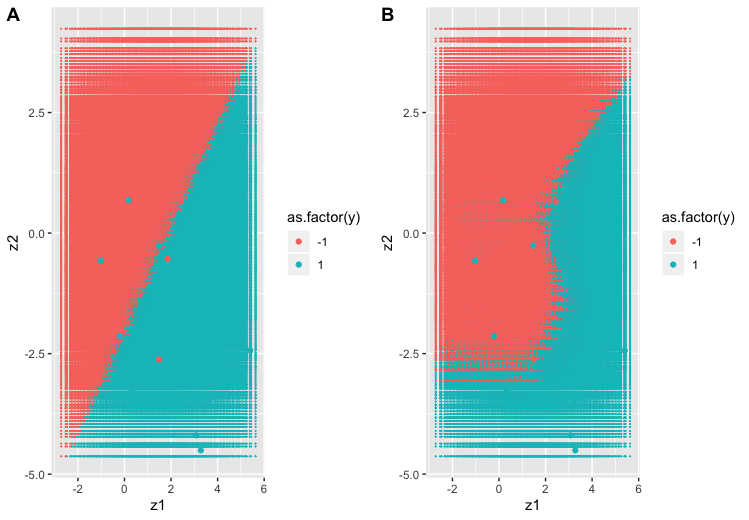
\includegraphics[width=.5\textwidth]{SMMK3.png}
\caption{\small $Z1$ and $Z2$ are projected axis from $\mX$ for visualization. Figure A shows the classification rule of SMM with linear kernel and Figure B shows SMM with polynomial kernel.}
\end{figure}
\vspace{-.5cm}


{\scriptsize Details in ``042320.pdf''.}
\end{frame}


\begin{frame}{Simulation: Probability function estimation}
\begin{figure}[H]
\centering
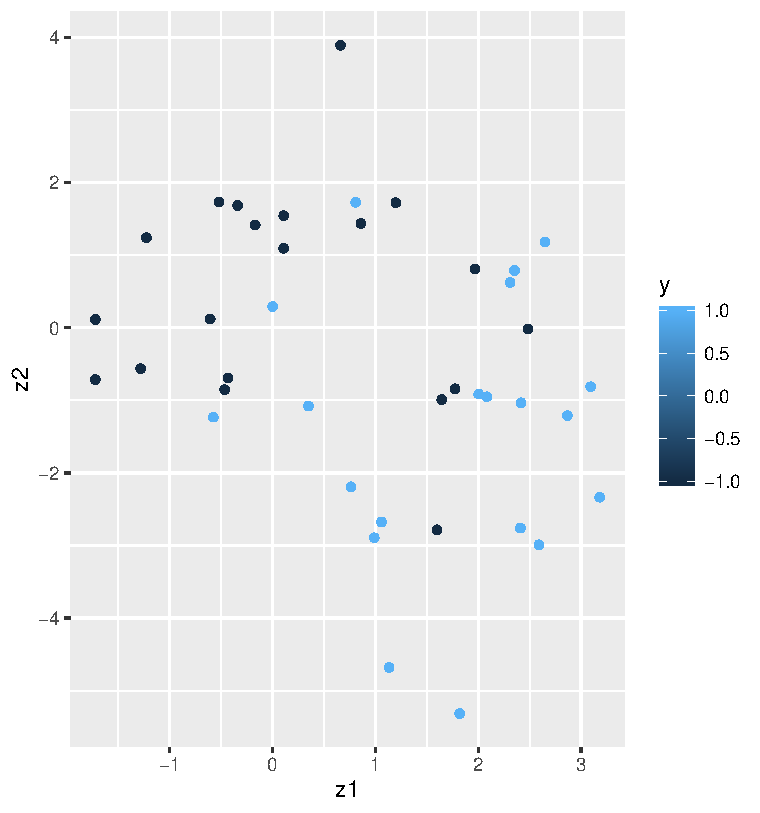
\includegraphics[width=.2\textwidth]{realization.pdf}
\caption{\scriptsize $Z1$ and $Z2$ are projected axis form $\mX$ for visualization.}
\end{figure}

\vspace{-.5cm}
\begin{figure}
    \centering
    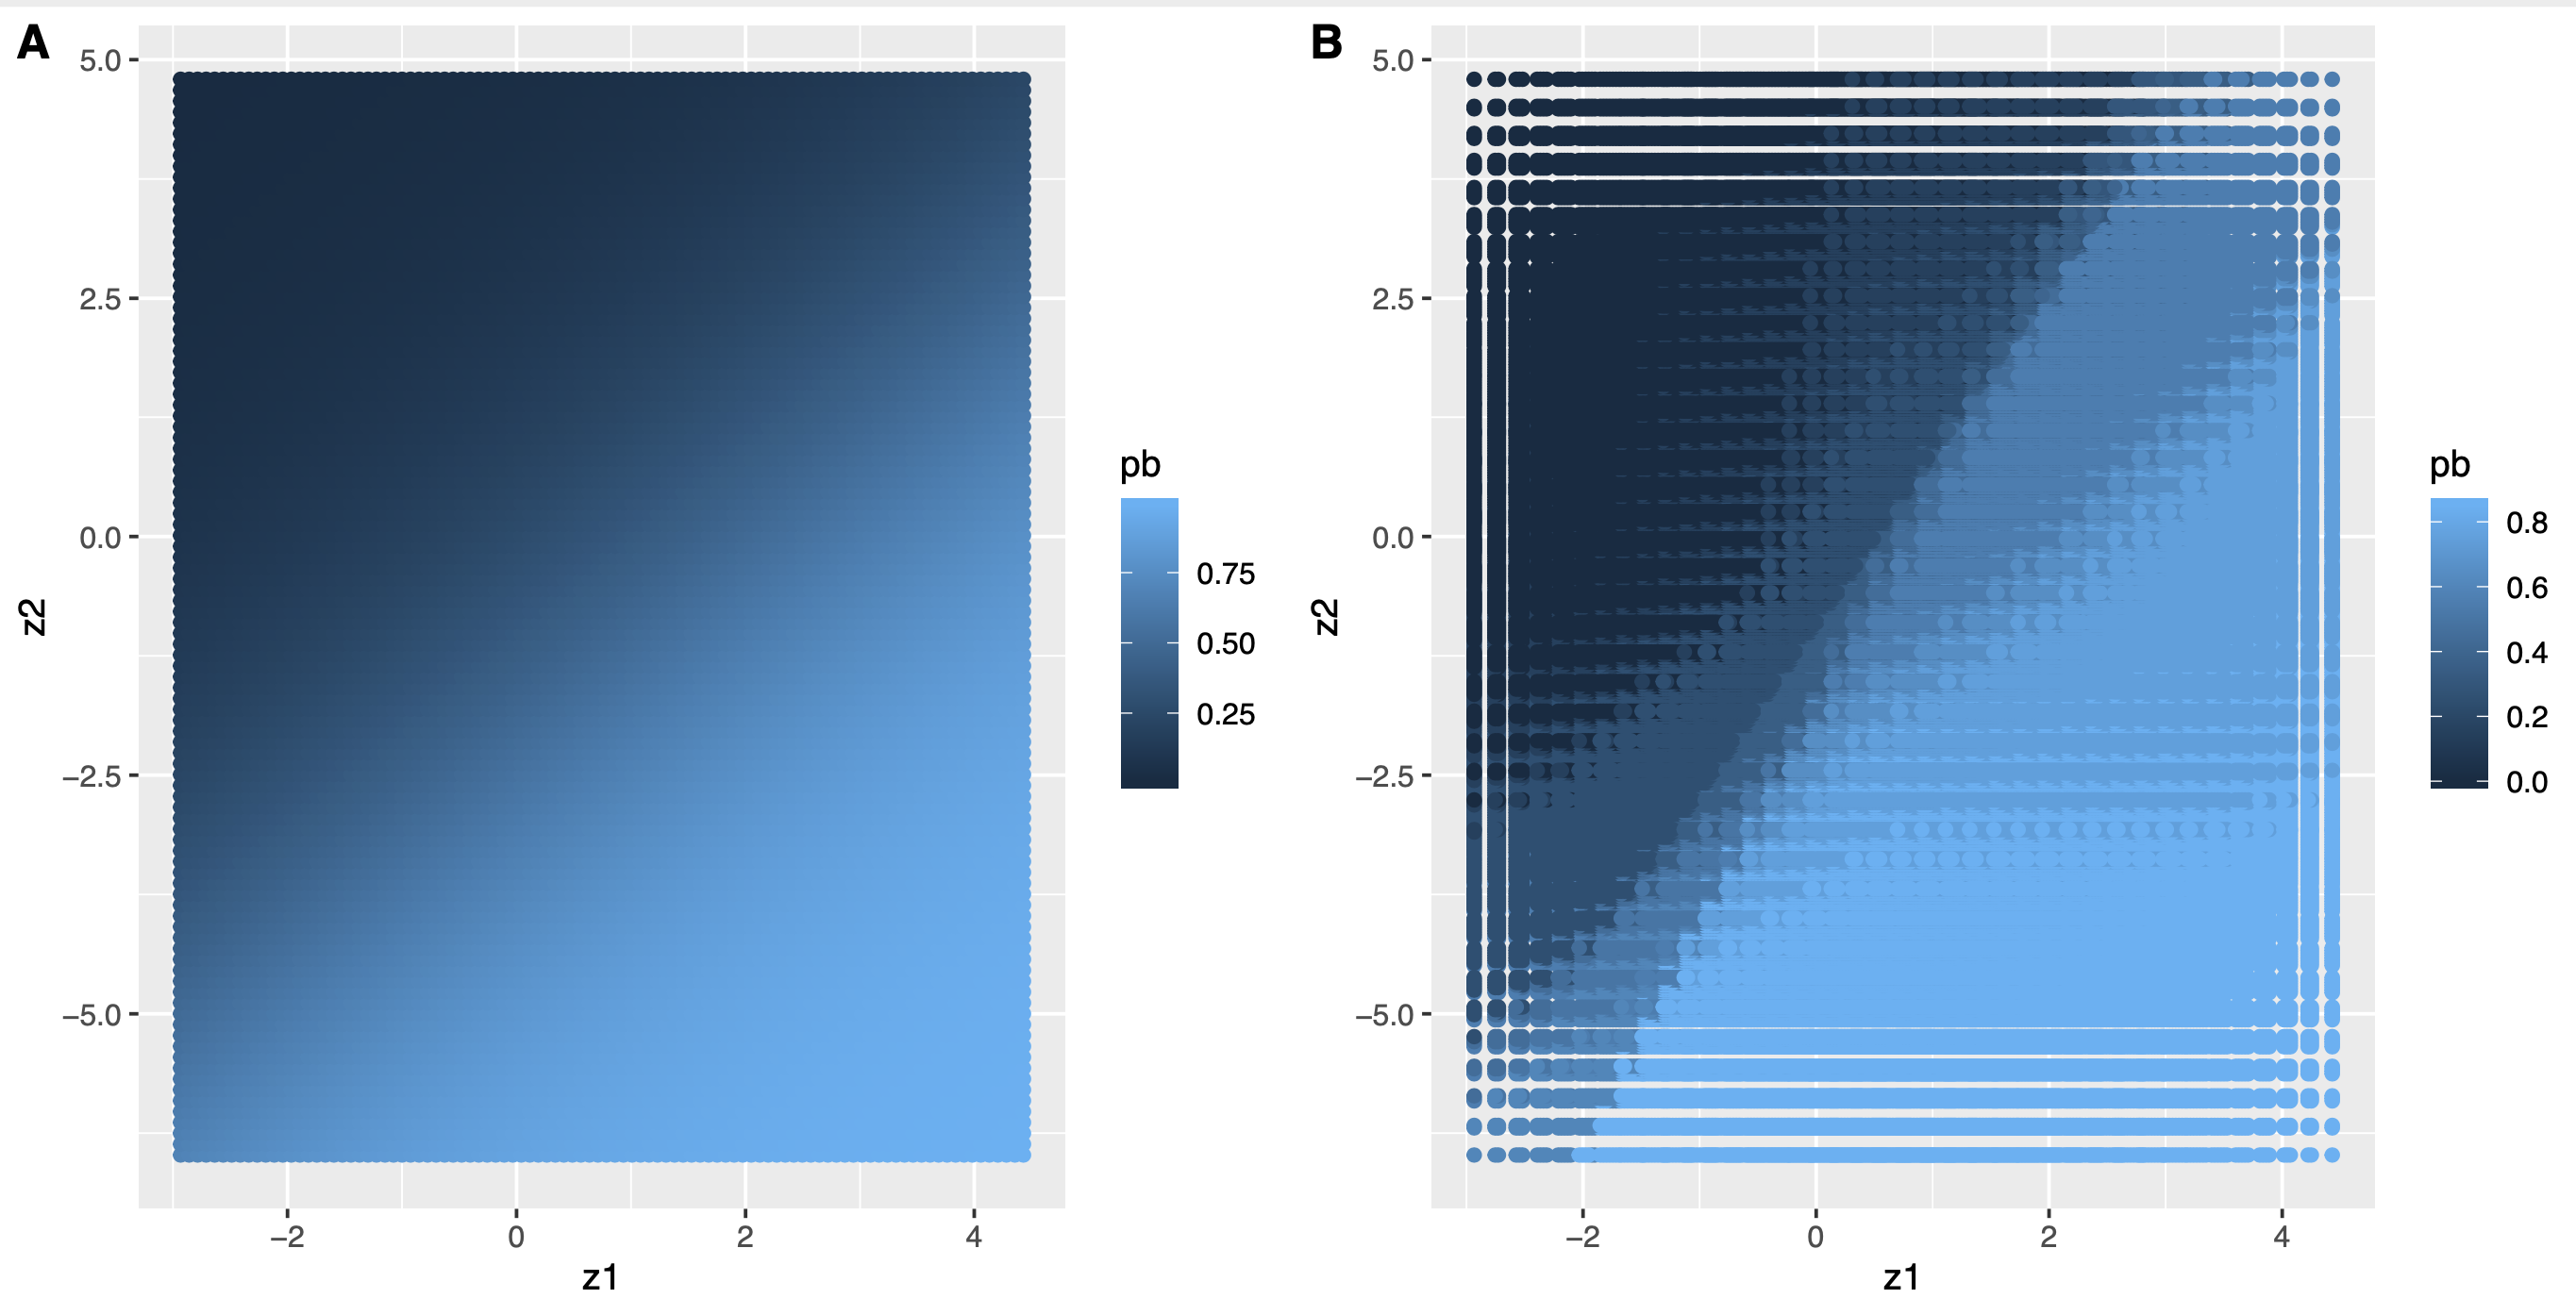
\includegraphics[width = 6 cm]{condpb.png}
    \label{fig:my_label}
    \caption{\scriptsize Figure A shows the true conditional probability of $y$ given $\mX\in\mathbb{R}^{2\times 2}$ (plotted on the first two principal directions). Figure B shows the estimated probability via low-rank SMM. }
\end{figure}
%{\scriptisize Figure A shows the true conditional probability of $y$ given $\mX\in\mathbb{R}^{2\times 2}$ (plotted on the first two principal directions). Figure B shows the estimated probability via low-rank SMM. }
{\scriptsize Details in ``042020.pdf''.}
\end{frame}





\section{Nonlinear learning with low-rank kernels}
\subsection{Nonlinear matrix-valued kernels}
\begin{frame}{Extension to nonlinear kernels}
\begin{itemize}
\item Let $\mX,\mX'\in\mathbb{R}^{d_1\times d_2}$ be a pair of matrices. Given a projection matrix $\mP\in\mathbb{R}^{r\times d_1}$, {\color{red}a linear low-rank kernel} is defined as
\begin{align}
\langle \mX, \mX' \rangle_{\mP}&\stackrel{\text{def}}{=} \langle {\color{red}\mP} \mX,\ {\color{red}\mP} \mX'\rangle\\
&= \text{trace}\left[\KeepStyleUnderBrace{\mX\mX'^T}_{\text{bilinear map}}\KeepStyleUnderBrace{\mP^T\mP}_{\text{low-rank projection}}\right].
\end{align}
\item Similarly, we propose {\color{red}a nonlinear low-rank kernel}
\begin{align}
\langle \mX, \mX' \rangle_{\text{$\mP$,h}}&\stackrel{\text{def}}{=} \langle {\color{red}\mP} h(\mX),\ {\color{red}\mP} h(\mX')\rangle\\
%&=\text{tr}(h(\mX)h^T(\mY) \mP^T_c\mP_c) 
&=\text{trace}\left[{\color{red}\mK(\mX,\mX')}\mP^T\mP\right],
\end{align}
where $h\colon \mathbb{R}^{d_1\times d_2}\mapsto \mathbb{R}^{d_1\times d_2'}$ denotes a nonlinear map between two matrix spaces, and $\mK(\mX,\mX')\stackrel{\text{def}}{=}h(\mX)h^T(\mX')\in\mathbb{R}^{d_1\times d_1}$ denotes the matrix product of mapped features. 
%\item For any classical kernel $K(\cdot,\cdot)$, we propose the matrix-valued kernel 
%\begin{align}
%\tK\colon \mathbb{R}^{d_1\times d_2}\times \mathbb{R}^{d_1\times d_2} &\mapsto \mathbb{R}^{d_2\times d_2}\\
%(\mX,\mY)&\mapsto [\tK(\mX, \mY)]_{i,j}=K(\mX[\colon,i], \mY[\colon,j]).
%\end{align}
\end{itemize}
\end{frame}


\begin{frame}{Nonlinear kernels for matrix predictors}
\begin{itemize}
\item Each entry of $\mK(\mX,\mX')$ is the inner product between two vectors. 
\item We refer to $\mK(\cdot,\ \cdot)\in\mathbb{R}^{d_1\times d_1}$ as the \emph{lifted (matrix-valued) kernel} induced by the nonlinear map $h$. 
\item Examples:
\begin{itemize}
\item Linear kernel: $\mK(\mX,\mX')=\mX\mX'^T$.
\item Polynomial kernel with degree $m$: $\mK(\mX,\mX')=(\mX\mX'^T+\lambda\mI)^{\circ m}$.
\item Gaussian kernel: the $(i,j)$-th entry of $\mK(\mX,\mX')$ is 
\[
\left[\mK(\mX,\mX')\right]_{(i,j)}=\exp\left\{-{1\over 2\sigma^2} \vectornorm{\mX[i,\colon]-\mX'[j,\colon]}^2\right\}
\]
for all $(i,j)\in[d_1]\times[d_1]$.
\end{itemize}
\item Implementation: (1) symmetrization trick; (2) A single projection matrix is enough to guide the optimization. Update at every other step. 
\item {\it Perhaps use a different name for $\mK$? Not really a kernel... 

$\mK(\mX,\mX')\neq \mK(\mX',\mX)$; $\mK(\mX, \mX')\neq \mK(\mX^T, \mX'^T)$.}

\end{itemize}
\end{frame}

\subsection{Nonlinear learning with matrix predictors}
\begin{frame}{Application of nonlinear kernels to matrix-based learning}
\begin{itemize}
\item Nonparametric classifier: $\text{sign}[\hat f(\cdot)]\colon \mathbb{R}^{d_1\times d_2}\mapsto\{-1,1\}$, where
\[
\hat f(\cdot)=\sum_i \hat \alpha_iy_i \text{tr}\left[\mK(\cdot,\ \mX_i)\hat \mP^T\hat \mP \right].
\]
\item Nonparametric regression:
\begin{align}
\hat{\mathbb{P}}(Y=1|\mX^{\text{new}})&={1\over H}\sum_{h\in[H]} \mathds{1}\left\{\mX^{\text{new}}\colon \text{sign}[\hat f_h(\mX^{\text{new}})]=1 \right\}
\end{align}
\item Nonlinear SDR, $Y\ind \mX \big| \phi(\mX)$, where 
\[
\phi(\mX)=h(\mX) \times_1\hat \mP_c\times_2 \hat \mP_r (??)
\]
\end{itemize}
\end{frame}

\subsection{Simulations}
\begin{frame}{Simulation: Linear vs.\ nonlinear classification}
\begin{itemize}
\item linearly separable, homoscedastic case: $d_1=10, d_2=8, r=3, N=100$
\begin{table}[h!]
    \centering
    \scalebox{0.8}{
\begin{tabular}{l|r|r|r|r|r|r}
\hline
  & 1st & 2nd & 3rd & 4th & 5th & average\\
\hline
SVM & 0.85 & 0.70 & 0.75 & 0.70 & 0.50 & 0.70\\
\hline
SMM & \color{red}0.90 & \color{red}0.90 & 0.75 & \color{red}0.80 & \color{red}0.85 & \color{red}0.84\\
\hline
SMM(polynomial) & 0.75 & 0.55 & \color{red}0.85 & 0.55 & 0.75 & 0.69\\
\hline
SMM(gaussian) & 0.65 & 0.50 &\color{red} 0.85 & 0.70 & 0.80 & 0.70\\
\hline
\end{tabular}}
    \caption{\scriptsize 1-MCR on 5 folded Cross validation(CV)}
    \label{tab:sim1.1}
\end{table}



\item Non-separable, heteroscedastic case: $d_1=d_2=2, \text{Cov}(\mX|y=-1)=4\text{Cov}(\mX|y=1)=4\mI_2$.
\begin{table}[h!]
    \centering
    \scalebox{0.8}{
\begin{tabular}{l|r|r|r}
\hline
  & sim 2.1 & sim 2.2 & sim 2.3\\
\hline
SVM & 0.76 & 0.735 & 0.860 \\
\hline
SMM & 0.75 & 0.740 &{\color{red} 0.865}\\
\hline
SMM(polynomial) & {\color{red}0.80} & {\color{red}0.750} & 0.785 \\
\hline
SMM(gaussian) & 0.71 & 0.745 & 0.830 \\
\hline
\end{tabular}}
    \caption{\scriptsize Averaged 1-MCR of 5 folded CV according to different methods.}
    \label{tab:cv}
\end{table}
\end{itemize}
{\scriptsize Details in ``042720.pdf''}
\end{frame}


\begin{frame}{Simulation: Nonlinear learning}
\begin{itemize}
\item Nonlinear classification
\begin{figure}[H]
\centering
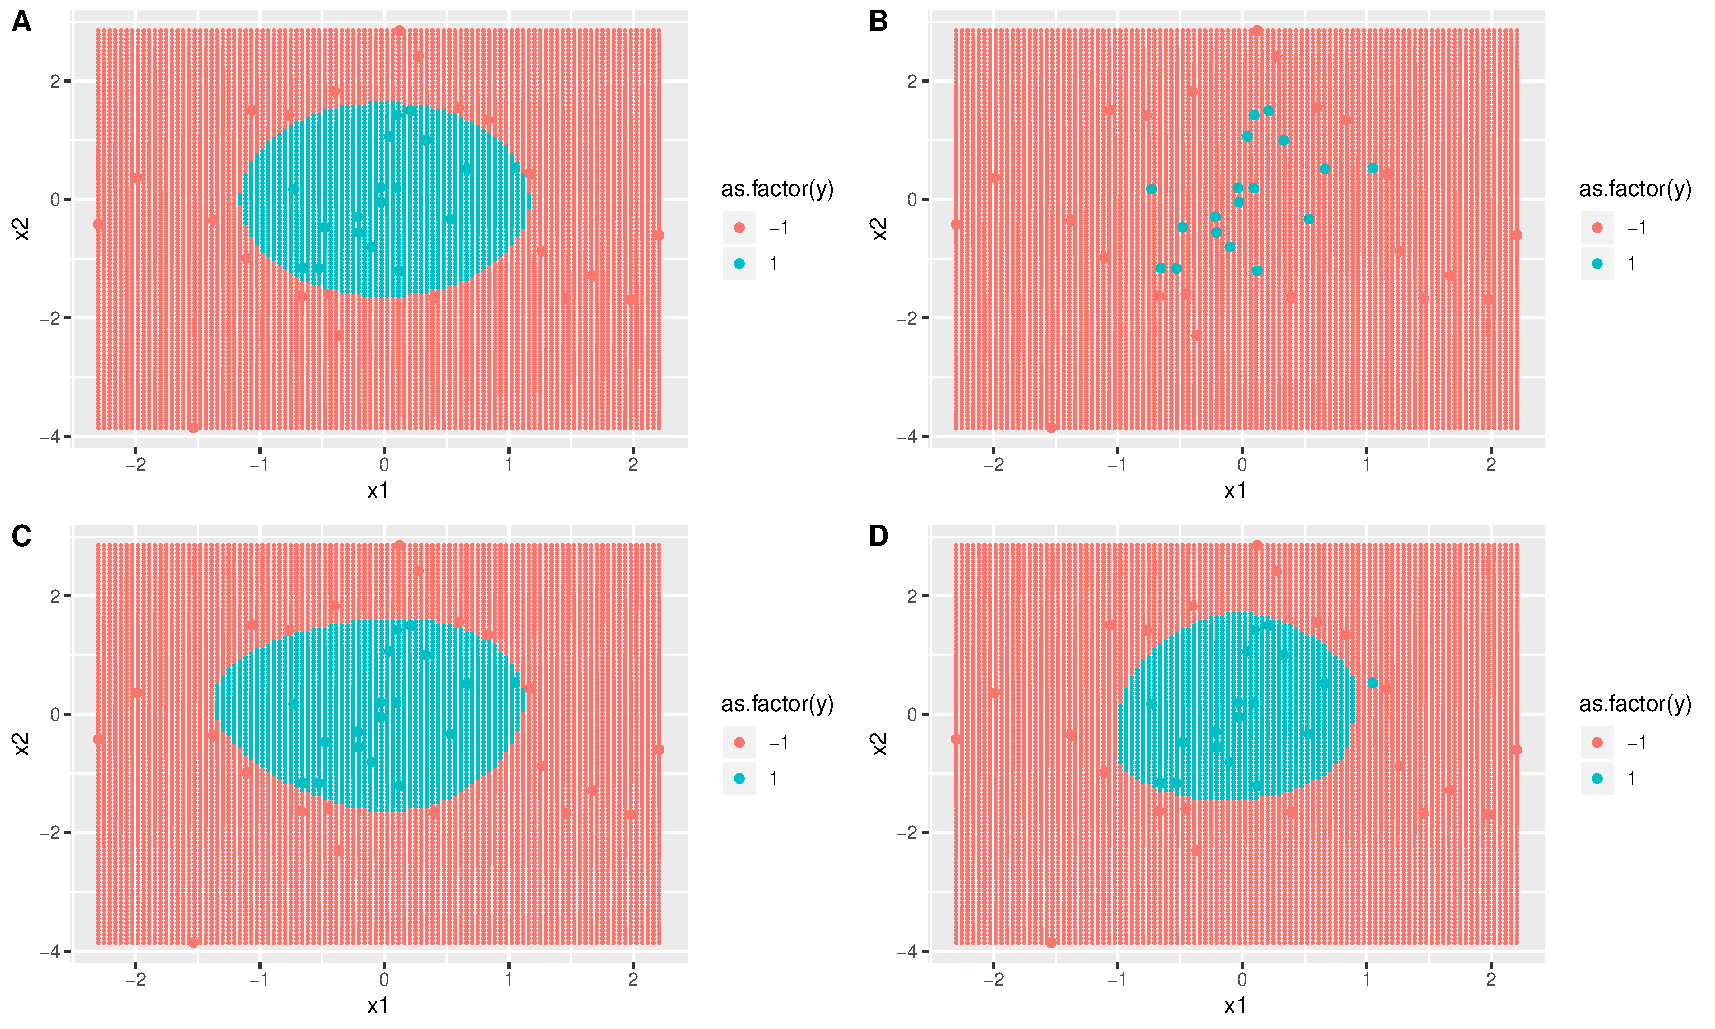
\includegraphics[width=.7\textwidth]{SMMK_boundary.pdf}
\caption{\scriptsize Subfigure A is true ellipsoid boundary. B is linear case boundary which assigns labels all 0. C and D show the boundary of polynomial and exponential kernel respectively.}
\end{figure}
\end{itemize}
\end{frame}


\begin{frame}{Simulation: Nonlinear learning (cont.)}
\begin{itemize}
\item Nonlinear probability estimation
\begin{figure}[H]
\centering
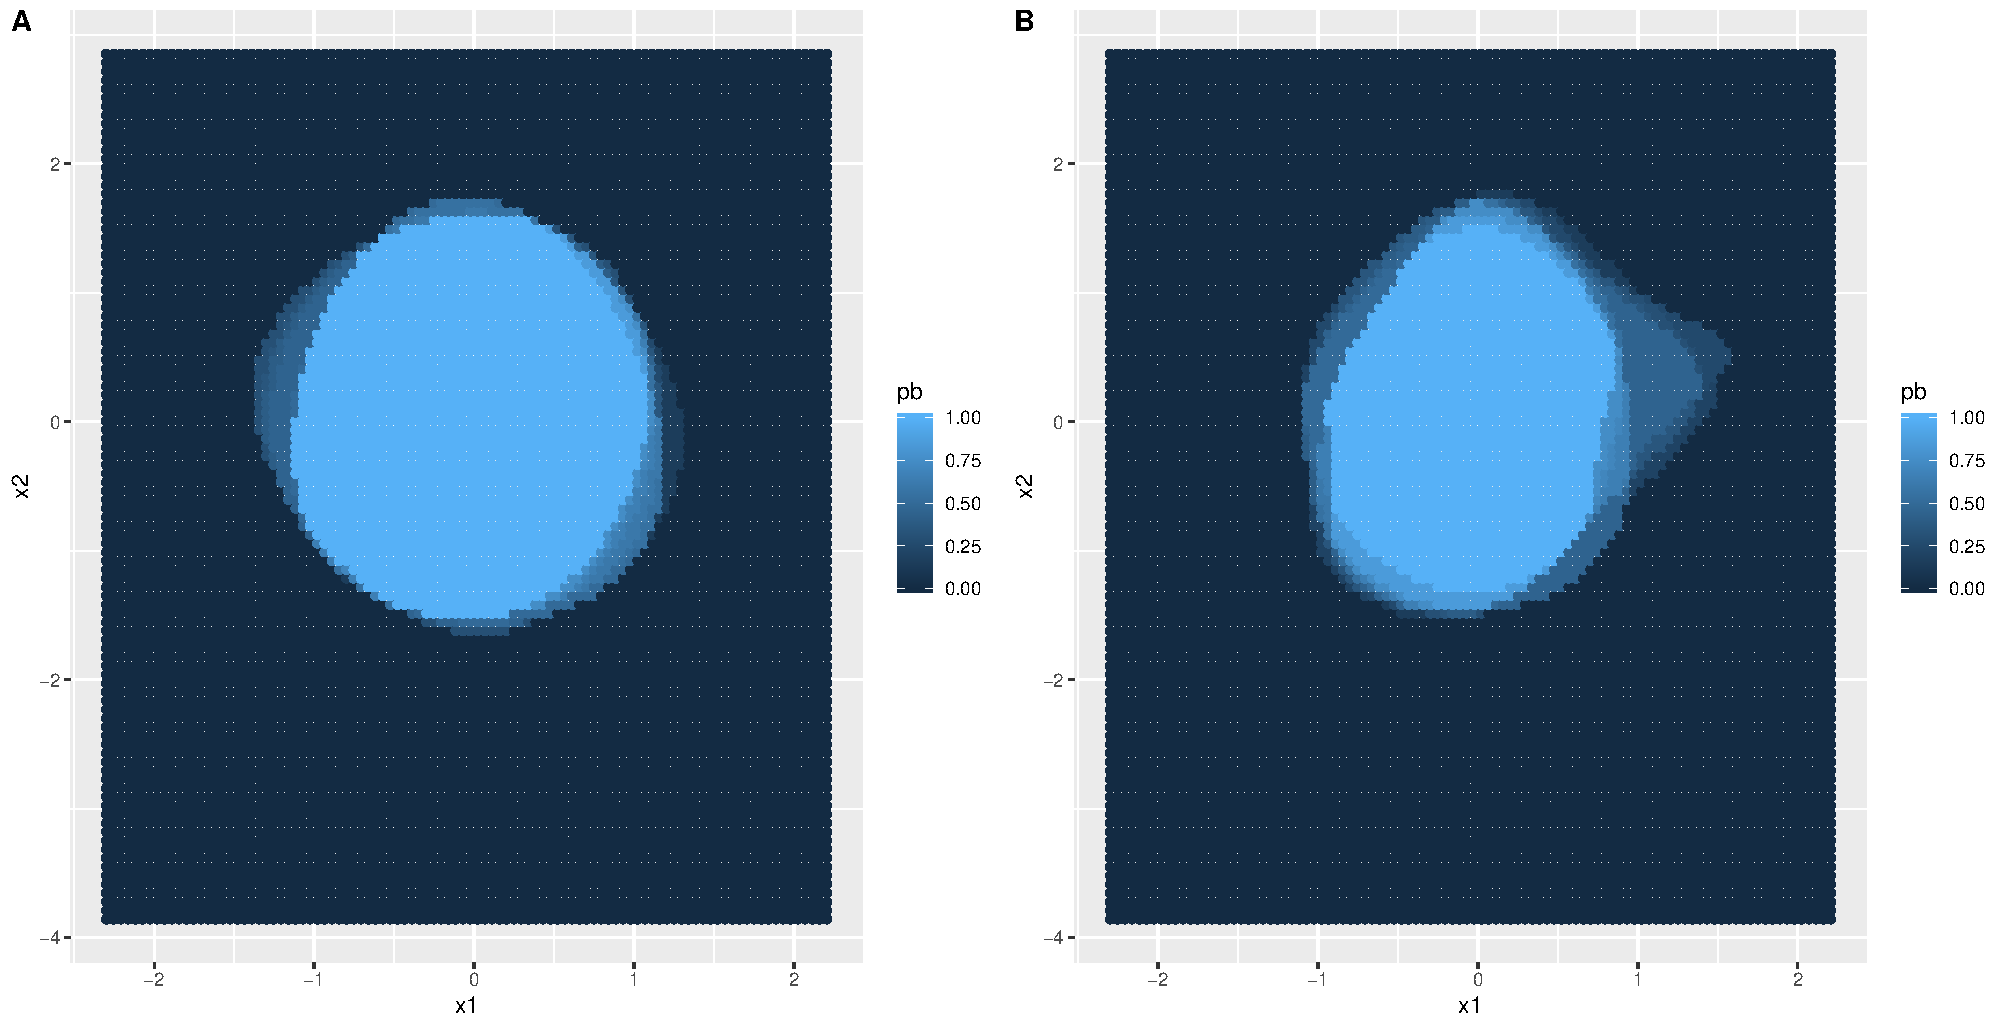
\includegraphics[width=.7\textwidth]{SMMK_condpb.pdf}
\caption{\scriptsize Figure A and B show the estimated probability with polynomial and exponential kernel respectively. }
\end{figure}
\end{itemize}
{\scriptsize Details in ``052120.pdf''}
\end{frame}


\begin{frame}{Summary}

\begin{itemize}
\item We have developed a robust nonparametric framework for classification, prediction and dimension reduction with {\color{red}matrix-valued predictors}. 

\vspace{.2cm}
\item The proposed {\color{red}low-rank projection kernel} achieves statistical efficiency and adaptability in high dimension regimes.
\vspace{.2cm}
\item Our method can be thought of as {\color{red}adaptive kernel learning} by jointly performing (nonlinear or linear) dimension reduction and classification/prediction. 
\vspace{.2cm}
\item {\color{red}Computational efficiency} can be further boosted by employing solution path algorithm and stochastic gradient descent. 
\end{itemize}
\end{frame}
\begin{frame}{Questions}
\begin{itemize}
\item [Regression] How does SVM-based learning compare to other nonparametric regression, such as local smoothing, K-NN, Neural Network?\\
\vspace{.4cm}
 $\Rightarrow$ SVM-based learning is essentially a kernel smoothing method. Neighborhood is defined by support vectors (c.f.~\eqref{eq:f}). Intuition? 
 \vspace{.2cm}
\item [SDR] How does SVM-based SDR compare to other SDR methods? 
\vspace{.2cm}
\item [Kernel] Connection between low-rank kernel vs.\ adaptive kernel, kernel learning, sum of rank-1 kernels?  
\vspace{.4cm}
\item Extend to higher-order tensors. Data-driven choice of $r$. 
\vspace{.4cm}
\item Real data analysis
\end{itemize}
\end{frame}
\bibliography{binary_tensor}
\end{document}
